\begin{figure}[h]
	\centering
	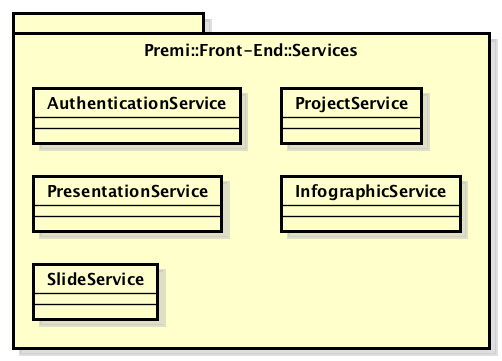
\includegraphics[width=0.7\linewidth]{img/premi_front_end_services}
	\caption[Premi::Front-End::Services]{Premi::Front-End::Services}
\end{figure}
Il package gestisce i services del front-end. Comunica con il model e i controller per creare le funzioni comuni ad essi e richiamarle. È inoltre il responsabile delle chiamate alle API REST del back-end per salvare e caricare i dati dal database.


\subsubsection{forgotPasswordService}
	\begin{figure}[h]
		\centering
		%		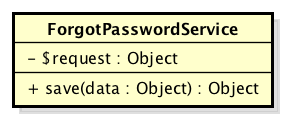
\includegraphics[width=0.6\linewidth]{img/premi_front_end_services_forgotpasswordservice}
		\caption[Premi::Front-End::Services::ForgotPasswordService]{Premi::Front-End::Services::ForgotPasswordService}
	\end{figure}
	
	\paragraph{Descrizione}
	Si occupa di gestire il processo di recupero password per l'autenticazione dell'utente.
	
	\paragraph{Utilizzo}
	Viene utilizzato per creare una risorsa collegata al servizio REST che permette il recupero della password dell'utente.
	
	\paragraph{Relazioni con le altre classi}
	\begin{itemize}
		\item \textbf{\textit{OUT} AuthenticationCtrl}:\\
			Classe che gestisce le operazioni per l'autenticazione dell'utente al sistema.
	\end{itemize}
	
	\paragraph{Attributi}
	\begin{itemize}
		\item \textbf{- \$request: Object}:\\
		Campo dati contenente la route per la chiamata al servizio REST specifico del servizio.
	\end{itemize}	
	
	\paragraph{Metodi}
	\begin{itemize}
		\item \textbf{+ save(data: Object)}:\\
		Metodo che richiama la funzione PUT collegata alla risorsa e permette di eseguire la chiamata alla funzione definita nella parte di backend la quale avvia il processo di recupero password, inviando una mail all'indirizzo passato attraverso il parametro della funzione.\\
		\textbf{Parametri:}\\
		\begin{itemize}
			\item \textit{data: Object}: parametro di un oggetto JSON che contiene l'indirizzo email inserito nella view.
		\end{itemize}
	\end{itemize}
	
	
\subsubsection{indexService}
	\begin{figure}[h]
		\centering
		%		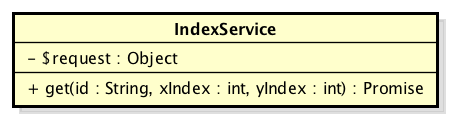
\includegraphics[width=0.6\linewidth]{img/premi_front_end_services_indexservice}
		\caption[Premi::Front-End::Services::IndexService]{Premi::Front-End::Services::IndexService}
	\end{figure}
	
	\paragraph{Descrizione}
	Si occupa di gestire le operazioni riguardanti gli indici delle slide.
	
	\paragraph{Utilizzo}
	Viene utilizzato per creare una risorsa collegata al servizio REST che permette di gestire le operazioni riguardanti gli indici delle slide.
	
	\paragraph{Relazioni con le altre classi}
	\begin{itemize}
		\item \textbf{\textit{OUT} SlideServiceCtrl}:\\
			Classe che gestisce le operazioni riguardanti le slide di un progetto.
	\end{itemize}
	
	\paragraph{Attributi}
	\begin{itemize}
		\item \textbf{- \$request: Object}:\\
			Campo dati contenente la route per la chiamata al servizio REST specifico del servizio.
	\end{itemize}	
	
	\paragraph{Metodi}
	\begin{itemize}
		\item \textbf{+ get(id: String, xIndex:int, yIndex:y): Promise}:\\
			Metodo che richiama la funzione GET collegata alla risorsa e permette di ottenere la slide avente x e y corrispondenti ai parametri passati. Il metodo ritorna una promessa la quale, se la chiamata ha esito positivo, conterrà un oggetto avente l'id della slide.\\
		\begin{itemize}
			\item \textit{id: String}: parametro di una stringa contenente l'id del progetto sul quale eseguire la funzione;
			\item \textit{xIndex: int}: parametro di un intero rappresentate la coordinata x della slide richiesta;
			\item \textit{yIndex: int}: parametro di un intero rappresentate la coordinata y della slide richiesta.
		\end{itemize}
	\end{itemize}


\subsubsection{loginService}
	\begin{figure}[h]
		\centering
%		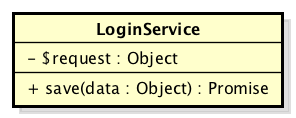
\includegraphics[width=0.6\linewidth]{img/premi_front_end_services_loginservice}
		\caption[Premi::Front-End::Services::LoginService]{Premi::Front-End::Services::LoginService}
	\end{figure}

	\paragraph{Descrizione}
	Si occupa di gestire il processo di login dell'utente.
	
	\paragraph{Utilizzo}
	Viene utilizzato per creare una risorsa collegata al servizio REST che permette l'autenticazione dell'utente al sistema.
	
	\paragraph{Relazioni con le altre classi}
	\begin{itemize}
		\item \textbf{\textit{OUT} AuthenticationCtrl}:\\
		Classe che gestisce le operazioni per l'autenticazione dell'utente al sistema.
	\end{itemize}
	
	\paragraph{Attributi}
	\begin{itemize}
		\item \textbf{- \$request: Object}:\\
			Campo dati contenente la route per la chiamata al servizio REST specifico del servizio.
	\end{itemize}	
	
	\paragraph{Metodi}
	\begin{itemize}
		\item \textbf{+ save(data: Object): Promise}:\\
			Metodo che richiama la funzione PUT collegata alla risorsa e permette di eseguire il login dell'utente al sistema. Il metodo ritorna una promessa la quale, se ha esito positivo, verrà analizzata per ottenere lo username dell'utente o il messaggio di errore. \\
			\textbf{Parametri:}\\
			\begin{itemize}
				\item \textit{data: Object}: parametro di un oggetto JSON che contiene il nome utente e la password inseriti nella view e necessari per l'autenticazione al sistema.
			\end{itemize}
	\end{itemize}
	
	
\subsubsection{logoutService}
	\begin{figure}[h]
		\centering
%		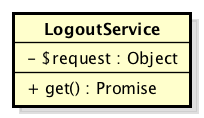
\includegraphics[width=0.6\linewidth]{img/premi_front_end_services_logoutservice}
		\caption[Premi::Front-End::Services::LogoutService]{Premi::Front-End::Services::LogoutService}
	\end{figure}
	
	\paragraph{Descrizione}
	Si occupa di gestire il processo di logout dell'utente.
	
	\paragraph{Utilizzo}
	Viene utilizzato per creare una risorsa collegata al servizio REST che permette l'autenticazione dell'utente al sistema.
	
	\paragraph{Relazioni con le altre classi}
	\begin{itemize}
		\item \textbf{\textit{OUT} AuthenticationCtrl}:\\
		Classe che gestisce le operazioni per l'autenticazione dell'utente al sistema.
	\end{itemize}
	
	\paragraph{Attributi}
	\begin{itemize}
		\item \textbf{- \$request: Object}:\\
		Campo dati contenente la route per la chiamata al servizio REST specifico del servizio.
	\end{itemize}	
	
	\paragraph{Metodi}
	\begin{itemize}
		\item \textbf{+ get(): Promise}:\\
		Metodo che richiama la funzione GET collegata alla risorsa e permette di eseguire il logout dell'utente. Il metodo ritorna una promessa e porta all'aggiornamento della pagina per il reset delle variabili si \$scope.
	\end{itemize}
	
	
\subsubsection{presentationService}
	\begin{figure}[h]
		\centering
		%		\includegraphics[width=0.6\linewidth]{img/premi_front_end_services_searchbypresentationservice}
		\caption[Premi::Front-End::Services::PresentationService]{Premi::Front-End::Services::PresentationService}
	\end{figure}
	
	\paragraph{Descrizione}
	Si occupa di gestire le operazioni riguardanti la presentazione di un progetto.
	
	\paragraph{Utilizzo}
	Viene utilizzato per creare una risorsa collegata al servizio REST che permette di gestire le operazioni sulle presentazioni, cioè di caricarle dal backend oppure di salvarle nel database.
	
	\paragraph{Relazioni con le altre classi}
	\begin{itemize}
		\item \textbf{\textit{OUT} PresentationCtrl}:\\
		Classe che gestisce le operazioni di visualizzazione di una presentazione;
		\item \textbf{\textit{OUT} PresentationEditorCtrl}:\\
			Classe che gestisce le operazioni modifica di una presentazione.
	\end{itemize}
	
	\paragraph{Attributi}
	\begin{itemize}
		\item \textbf{- \$request: Object}:\\
		Campo dati contenente la route per la chiamata al servizio REST specifico del servizio.
	\end{itemize}	
	
	\paragraph{Metodi}
	\begin{itemize}
		\item \textbf{+ query(id: String): Promise}:\\
			Metodo che richiama la funzione GET collegata alla risorsa e permette di caricare la presentazione dal database. Il metodo ritorna una promessa la quale, se la chiamata ha esito positivo, conterrà la presentazione con tutte le rispettive slide.\\
		\item \textbf{+ update(id: String, theme:String, transition:String): Promise}:\\
			Metodo che richiama la funzione POST collegata alla risorsa e permette di salvare la presentazione aggiornando i dati, anche quelli riguardanti il tema e la transizione tra le slide passati per parametro. Il metodo ritorna una promessa la quale, se la chiamata ha esito positivo, conterrà il valore \textit{true}.\\
		\textbf{Parametri:}\\
		\begin{itemize}
			\item \textit{id: String}: parametro di una stringa contenente l'id della presentazione sulla quale eseguire le operazioni;
			\item \textit{theme: String}: parametro di una stringa contenente il nome del tema da applicare alla presentazione;
			\item \textit{transition: String}: parametro di una stringa contenente il nome della transizione da applicare alla presentazione.
		\end{itemize}
	\end{itemize}
	
	
\subsubsection{projectService}
	\begin{figure}[h]
		\centering
		%		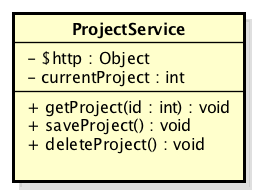
\includegraphics[width=0.6\linewidth]{img/premi_front_end_services_projectservice}
		\caption[Premi::Front-End::Services::ProjectService]{Premi::Front-End::Services::ProjectService}
	\end{figure}
	
	\paragraph{Descrizione}
	Si occupa di gestire le operazioni riguardanti uno specifico progetto di un utente.
	
	\paragraph{Utilizzo}
	Viene utilizzato per creare una risorsa collegata al servizio REST che permette di gestire le operazioni sul progetto, cioè di caricarlo o eliminarli dal database.
	
	\paragraph{Relazioni con le altre classi}
	\begin{itemize}
		\item \textbf{\textit{OUT} ProjectCtrl}:\\
			Classe che gestisce le operazioni riguardanti i progetti;
	\end{itemize}
	
	\paragraph{Attributi}
	\begin{itemize}
		\item \textbf{- \$request: Object}:\\
		Campo dati contenente la route per la chiamata al servizio REST specifico del servizio.
	\end{itemize}	
	
	\paragraph{Metodi}
	\begin{itemize}
		\item \textbf{+ delete(id: String): Promise}:\\
			Metodo che richiama la funzione DELETE collegata alla risorsa e permette di rimuovere il progetto e tutto il suo contenuto dal database. Il metodo ritorna una promessa la quale, se la chiamata ha esito positivo, conterrà il valore \textit{true}.\\
		\item \textbf{+ update(id: String, data:Object): Promise}:\\
			Metodo che richiama la funzione PUT collegata alla risorsa e permette di aggiornare i dati del progetto passati per parametro. Il metodo ritorna una promessa la quale, se la chiamata ha esito positivo, conterrà il valore \textit{true}.\\
		\textbf{Parametri:}\\
		\begin{itemize}
			\item \textit{id: String}: parametro di una stringa contenente l'id del progetto sul quale eseguire le operazioni;
			\item \textit{data: Object}: parametro di un oggetto contenente i dati del progetto da aggiornare.
		\end{itemize}
	\end{itemize}


\subsubsection{projectsService}
	\begin{figure}[h]
		\centering
		%		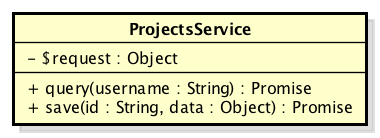
\includegraphics[width=0.6\linewidth]{img/premi_front_end_services_projectsservice}
		\caption[Premi::Front-End::Services::ProjectsService]{Premi::Front-End::Services::ProjectsService}
	\end{figure}
	
	\paragraph{Descrizione}
	Si occupa di gestire le operazioni riguardanti i progetti.
	
	\paragraph{Utilizzo}
	Viene utilizzato per creare una risorsa collegata al servizio REST che permette di gestire le operazioni sui progetti, cioè di caricarli o eliminarli dal database.
	
	\paragraph{Relazioni con le altre classi}
	\begin{itemize}
		\item \textbf{\textit{OUT} MyProjectsCtrl}:\\
			Classe che gestisce le operazioni riguardanti i progetti personali di un utente;
		\item \textbf{\textit{OUT} ProjectCtrl}:\\
			Classe che gestisce le operazioni riguardanti i progetti;
		\item \textbf{\textit{OUT} SearchCtrl}:\\
			Classe che gestisce le operazioni di ricerca. Viene usato per caricare i progetti trovati.
	\end{itemize}
	
	\paragraph{Attributi}
	\begin{itemize}
		\item \textbf{- \$request: Object}:\\
		Campo dati contenente la route per la chiamata al servizio REST specifico del servizio.
	\end{itemize}	
	
	\paragraph{Metodi}
	\begin{itemize}
		\item \textbf{+ query(username: String): Promise}:\\
			Metodo che richiama la funzione GET collegata alla risorsa e permette di caricare i progetti dell'utente con username passato per parametro e i rispettivi contenuti dal database. Il metodo ritorna una promessa la quale, se la chiamata ha esito positivo, conterrà un oggetto avente il progetto e i suoi dati.\\
		\item \textbf{+ save(id: String, data:Object): Promise}:\\
			Metodo che richiama la funzione POST collegata alla risorsa e permette di creare un nuovo progetto con i dati passati per parametro. Il metodo ritorna una promessa la quale, se la chiamata ha esito positivo, conterrà il valore \textit{true}.\\
		\textbf{Parametri:}\\
		\begin{itemize}
			\item \textit{username: String}: parametro di una stringa contenente lo username dell'utente;
			\item \textit{id: String}: parametro di una stringa contenente l'id del progetto sul quale eseguire le operazioni;
			\item \textit{data: Object}: parametro di un oggetto contenente i dati necessari per creare il progetto, quali ad esempio il nome.
		\end{itemize}
	\end{itemize}
	
	
\subsubsection{searchByUserService}
	\begin{figure}[h]
		\centering
		%		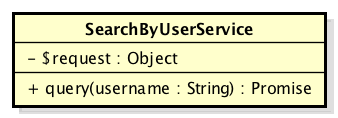
\includegraphics[width=0.6\linewidth]{img/premi_front_end_services_searchbyuserservice}
		\caption[Premi::Front-End::Services::SearchByUserService]{Premi::Front-End::Services::SearchByUserService}
	\end{figure}
	
	\paragraph{Descrizione}
	Si occupa di gestire il processo di ricerca del sistema.
	
	\paragraph{Utilizzo}
	Viene utilizzato per creare una risorsa collegata al servizio REST che permette la ricerca nel sistema attraverso il nome utente.
	
	\paragraph{Relazioni con le altre classi}
	\begin{itemize}
		\item \textbf{\textit{OUT} HomePageCtrl}:\\
		Classe che gestisce le operazioni di reindirizzamento tra le pagine dall'applicazione e le operazioni di ricerca.
	\end{itemize}
	
	\paragraph{Attributi}
	\begin{itemize}
		\item \textbf{- \$request: Object}:\\
		Campo dati contenente la route per la chiamata al servizio REST specifico del servizio.
	\end{itemize}	
	
	\paragraph{Metodi}
	\begin{itemize}
		\item \textbf{+ query(username: String): Promise}:\\
		Metodo che richiama la funzione GET collegata alla risorsa e permette di eseguire la ricerca nel sistema attraverso lo username di un utente. Il metodo ritorna una promessa la quale, se la chiamata ha esito positivo, conterrà un array con gli utenti risultato della ricerca, ognuno dei quali avrà le informazioni necessarie per recuperare i rispettivi progetti da analizzare.\\
		\textbf{Parametri:}\\
		\begin{itemize}
			\item \textit{username: String}: parametro di una stringa contenente il nome utente da cercare inserito nella view.
		\end{itemize}
	\end{itemize}


\subsubsection{searchByProjectService}
	\begin{figure}[h]
		\centering
		%		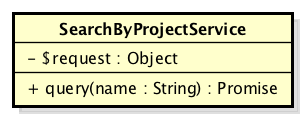
\includegraphics[width=0.6\linewidth]{img/premi_front_end_services_searchbyprojectservice}
		\caption[Premi::Front-End::Services::SearchByProjectService]{Premi::Front-End::Services::SearchByProjectService}
	\end{figure}
	
	\paragraph{Descrizione}
	Si occupa di gestire il processo di ricerca del sistema.
	
	\paragraph{Utilizzo}
	Viene utilizzato per creare una risorsa collegata al servizio REST che permette la ricerca nel sistema attraverso il nome del progetto.
	
	\paragraph{Relazioni con le altre classi}
	\begin{itemize}
		\item \textbf{\textit{OUT} HomePageCtrl}:\\
		Classe che gestisce le operazioni di reindirizzamento tra le pagine dall'applicazione e le operazioni di ricerca.
	\end{itemize}
	
	\paragraph{Attributi}
	\begin{itemize}
		\item \textbf{- \$request: Object}:\\
		Campo dati contenente la route per la chiamata al servizio REST specifico del servizio.
	\end{itemize}	
	
	\paragraph{Metodi}
	\begin{itemize}
		\item \textbf{+ query(name: String): Promise}:\\
		Metodo che richiama la funzione GET collegata alla risorsa e permette di eseguire la ricerca nel sistema attraverso il nome di un progetto. Il metodo ritorna una promessa la quale, se la chiamata ha esito positivo, conterrà un array con i dati relativi ai progetti risultato della ricerca.\\
		\textbf{Parametri:}\\
		\begin{itemize}
			\item \textit{name: String}: parametro di una stringa contenente il nome del progetto da cercare inserito nella view.
		\end{itemize}
	\end{itemize}
	
	
\subsubsection{signupService}
	\begin{figure}[h]
		\centering
%		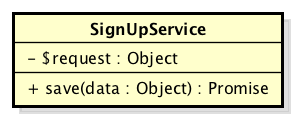
\includegraphics[width=0.6\linewidth]{img/premi_front_end_services_signupservice}
		\caption[Premi::Front-End::Services::SignupService]{Premi::Front-End::Services::SignupService}
	\end{figure}
	
	\paragraph{Descrizione}
	Si occupa di gestire il processo di registrazione dell'utente.
	
	\paragraph{Utilizzo}
	Viene utilizzato per creare una risorsa collegata al servizio REST che permette l'autenticazione dell'utente al sistema.
	
	\paragraph{Relazioni con le altre classi}
	\begin{itemize}
		\item \textbf{\textit{OUT} AuthenticationCtrl}:\\
		Classe che gestisce le operazioni per l'autenticazione dell'utente al sistema.
	\end{itemize}
	
	\paragraph{Attributi}
	\begin{itemize}
		\item \textbf{- \$request: Object}:\\
		Campo dati contenente la route per la chiamata al servizio REST specifico del servizio.
	\end{itemize}	
	
	\paragraph{Metodi}
	\begin{itemize}
		\item \textbf{+ save(data: Object): Promise}:\\
		Metodo che richiama la funzione PUT collegata alla risorsa e permette di eseguire la registrazione dell'utente al sistema. Il metodo ritorna una promessa la quale, se la chiamata ha esito positivo, verrà analizzata per ottenere la conferma di avvenuta registrazione o altrimenti, l'array contenenti gli errori commessi nell'inserimento dei dati.\\
		\textbf{Parametri:}\\
		\begin{itemize}
			\item \textit{data: Object}: parametro di un oggetto JSON che contiene tutte le credenziali necessarie inserite nella view per registrarsi come nuovo utente al sistema.
		\end{itemize}
	\end{itemize}


\subsubsection{slideService}
	\begin{figure}[h]
		\centering
		%		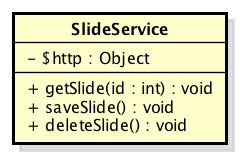
\includegraphics[width=0.6\linewidth]{img/premi_front_end_services_slideservice}
		\caption[Premi::Front-End::Services::SlideService]{Premi::Front-End::Services::SlideService}
	\end{figure}
	
	\paragraph{Descrizione}
	Si occupa di gestire le operazioni di una slide.
	
	\paragraph{Utilizzo}
	Viene utilizzato per creare una risorsa collegata al servizio REST che permette di modificare una slide. Dà la possiblità di creare, caricare, salvare e eliminare una slide dal database.
	
	\paragraph{Relazioni con le altre classi}
	\begin{itemize}
		\item \textbf{\textit{OUT} SlideEditorCtrl}:\\
			Classe che gestisce le operazioni di modifica di una slide.
	\end{itemize}
	
	\paragraph{Attributi}
	\begin{itemize}
		\item \textbf{- \$request: Object}:\\
		Campo dati contenente la route per la chiamata al servizio REST specifico del servizio.
	\end{itemize}	
	
	\paragraph{Metodi}
	\begin{itemize}
		\item \textbf{+ get(id:String): Promise}:\\
			Metodo che richiama la funzione GET collegata alla risorsa e permette di ottenere la slide dal backend identificata dall'id passato come parametro. IL metodo ritorna una promessa contenente un oggetto JSON avente tutte le informazioni e i dati riguardanti la slide e i suoi componenti. Questo oggetto è pronto per essere passato all'apposito metodo di caricamento della slide;
		\item \textbf{+ save(xIndex:int, yIndex:int): Promise}:\\
			Metodo che richiama la funzione POST collegata alla risorsa e permette di creare una nuova slide avente le coordinate passate per parametro. Il metodo ritorna una promessa la quale, se la chiamata ha esito positivo, conterrà l'id della nuova slide creata;\\
		\item \textbf{+ update(id:String, xIndex:int, yIndex:int, components:JSON, background:String, slideSVG:SVG):Promise}\\
			Metodo che richiama la funzione PUT collegata alla risorsa e permette di aggiornare una slide già creata (identificata dal parametro id). Con questa chiamata è possibile passare le coordinate aggiornate, i componenti della slide, il colore di sfondo e l'SVG rappresentante la slide stessa. Il metodo ritorna una promessa che conterrà \textit{true} se l'esito del salvataggio è positivo;
		\item \textbf{+ delete(id:String):Promise}\\
			Metodo che richiama la funzione DELETE collegata alla risorsa e permette di eliminare la slide con id passato per parametro. Il metodo ritorna una promessa che conterrà \textit{true} se l'esito del salvataggio è positivo.
			
		\textbf{Parametri:}\\
		\begin{itemize}
			\item \textit{background: String}: parametro di una stringa che contiene il codice del colore di sfondo della slide;
			\item \textit{components: JSON}: parametro di un oggetto JSON contenente tutti i componenti inclusi nella slide;
			\item \textit{id: String}: parametro di una stringa contenente l'id del progetto sul quale eseguire la funzione;
			\item \textit{slideSVG: SVG}: parametro di un oggetto SVG che contiene la rappresentazione della slide in SVG;
			\item \textit{xIndex: int}: parametro di un intero rappresentate la coordinata x della slide richiesta;
			\item \textit{yIndex: int}: parametro di un intero rappresentate la coordinata y della slide richiesta.
		\end{itemize}
	\end{itemize}
	
	
\subsubsection{userService}
	\begin{figure}[h]
		\centering
		%		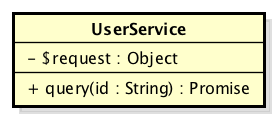
\includegraphics[width=0.6\linewidth]{img/premi_front_end_services_userservice}
		\caption[Premi::Front-End::Services::UserService]{Premi::Front-End::Services::UserService}
	\end{figure}
	
	\paragraph{Descrizione}
	Si occupa di gestire le operazioni riguardanti un utente.
	
	\paragraph{Utilizzo}
	Viene utilizzato per creare una risorsa collegata al servizio REST che permette di gestire le operazioni riguardanti un utente, quali il recupero dei suoi dati.
	
	\paragraph{Relazioni con le altre classi}
	\begin{itemize}
		\item \textbf{\textit{OUT} MyAccountCtrl}:\\
			Classe che gestisce la rappresentazione dei dati di un utente.
	\end{itemize}
	
	\paragraph{Attributi}
	\begin{itemize}
		\item \textbf{- \$request: Object}:\\
		Campo dati contenente la route per la chiamata al servizio REST specifico del servizio.
	\end{itemize}	
	
	\paragraph{Metodi}
	\begin{itemize}
		\item \textbf{+ query(id:String): Promise}:\\
		Metodo che richiama la funzione GET collegata alla risorsa e permette di ottenere i dati relativi all'utente con id passato come parametro. Il metodo ritorna una promessa contenete tutti i dati dell'utente
		\textbf{Parametri:}\\
		\begin{itemize}
			\item \textit{id: String}: parametro di una stringa contenente l'id dell'utente.
		\end{itemize}
	\end{itemize}